\chapter{Ms. Pac-Man} \label{cap:ms-pacman}
\begin{figure}[H]
\centering
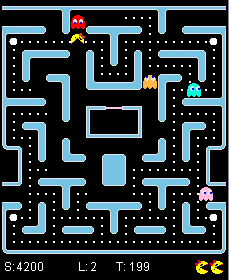
\includegraphics[width=6.5cm]{pacman}
\end{figure}

Ms. Pac-Man es un juego antológico desde su aparición en los arcades en el año 1981. Desde entonces han sido muchas las variantes de este clásico y sus diversos usos (recreacional, investigación, competición).
 
La versión del juego que vamos a utilizar, ``\textbf{\textit{Ms. Pac-Man Vs. Ghosts}}'' \cite{pacmanvsghostsTournamentPage} \cite{pacmanvsghostsGit}, está implementada por Philipp Rohlfshagen, basada en implementaciones previas de Simon Lucas y David Robles, los tres de la universidad de Essex, Reino Unido.


\section{Descripción del juego}
Las variantes del juego difieren mucho en cuanto a objetivos de juego y recompensas por los mismos, así como reglas a seguir. A continuación describimos la versión del juego que usamos en este trabajo.

El jugador o Pac-Man debe recorrer laberintos comiendo ``\textit{pills}'' y enfrentándose a cuatro fantasmas que intentarán perseguir a Pac-Man. Se dispone de 4 laberintos, todos con un ``\textit{lair}'' donde nacen y resucitan (cada nivel más rápidamente) los cuatro fantasmas tras ser comidos, y un punto en el que nace y resucita Pac-Man, el cual puede moverse por los laberintos cambiando su dirección en cualquier momento, siempre que la entrada dada por el jugador sea un movimiento válido (en otro caso continúa hacia delante en la dirección del último movimiento realizado exitosamente).
 
\blankline

Los laberintos son una serie de pasillos y cruces de caminos, repletos de \textit{pills}, y con cuatro ``\textit{power pills}'' cada uno. Las pills proporcionan puntos, y las power pills (con forma de pill agrandada) además permiten a Pac-Man comerse a los fantasmas durante un breve periodo de tiempo.

Todos los laberintos tienen una estructura toroidal (o \textit{wraparound}, esto es, al salir de los límites por un lado se aparece por el contrario, dando continuidad y dinamismo a la partida). Al comer Pac-Man una \textit{power pill}, puede comerse a los fantasmas durante un breve periodo de tiempo (siendo este periodo más corto en cada nivel), enviándolos al \textit{lair} y ganando puntos. Además, durante la duración del efecto de las \textit{power pills}, la velocidad de los fantasmas queda reducida a la mitad de la de Pac-Man. Las \textit{pills} y las \textit{power pills} también dan puntos, y se pasa al siguiente nivel cuando no queda ninguna de ambas.
 
No existen las frutas de la versión original del juego que aportan puntos adicionales.
Pac-Man tiene tres vidas (La inicial y dos más en reserva), pudiéndose obtener vidas adicionales cada 10.000 puntos.

Además, si tras 4000 iteraciones de la partida aún quedan \textit{pills} o \textit{power pills}, se pasa al siguiente nivel (considerando una iteración un intervalo de tiempo en el que tanto los fantasmas como Pac-Man hacen su movimiento y se actualiza el estado del tablero de juego). Este límite de tiempo se diseñó para evitar, en competiciones previas, que si un participante diseñaba una inteligencia artificial para controlar a los fantasmas, estos no pudieran bloquear una región del laberinto indefinidamente.
 
Los fantasmas tratan de impedir a Pac-Man completar cada laberinto y, al moverse (cuando no son comestibles) a la misma velocidad que este, emplean estrategias basadas en su superioridad numérica. Además, los fantasmas no pueden darse la vuelta (retroceder), con una excepción: turno a turno los fantasmas tienen una pequeña probabilidad de darse la vuelta forzosamente, por defecto 0.015\%.
 
La puntuación se obtiene con los siguientes cálculos (originales del código de competición):
\begin{itemize}
\item Comer pill: 10 puntos.
\item Comer power pill: 50 puntos.
\item Comer fantasma: 200 puntos, duplicándose el valor por cada fantasma comido en cadena (Si durante la duración de la misma \textit{power pill} se come un segundo fantasma, este vale 400; el siguiente 800, etc).
\end{itemize}

\section{Arquitectura para crear bots}
El código del juego viene preparado para facilitar a los concursantes diseñar sus bots, que han de implementar su código en la clase ``\textit{MyPacMan}'', con clases auxiliares en ``\textit{pacman/entries/pacman/}''. Dicha clase incluye el método a implementar, que ha de devolver el siguiente movimiento de Pac-Man en cada turno, pudiendo hacer consultas a las funciones de la clase ``\textit{Game}'', que contiene el estado del juego para realizar el más conveniente en cada caso.
 
La versión original trae como ejemplo una serie de controladores para los fantasmas, que vamos a usar para medir la ``calidad'' o ``cómo de buenos'' son los programas que generemos con gramáticas evolutivas. Son los siguientes:
\begin{itemize}
\item \textbf{Random Ghosts}. Los fantasmas toman direcciones aleatorias cada vez que llegan a una intersección y al salir del \textit{lair}.

\item \textbf{Starter Ghosts}. Versión de los fantasmas que consiste en: Alejarse de Pac-Man si está cerca de una \textit{power pill} o si el fantasma en concreto es comestible (por haberse comido Pac-Man una \textit{power pill} mientras él estaba vivo), o si no, con un 90\% de posibilidades dirigirse hacia Pac-Man y con un 10\% hacer un movimiento aleatorio entre los que sean posibles para el fantasma en ese momento.

\item \textbf{Aggressive Ghosts}. Cada vez que un fantasma llega a una intersección tiene una probabilidad determinada de o bien dirigirse hacia Pac-Man, o bien hacer un movimiento aleatorio.

\item \textbf{Legacy}. \textit{Legacy} diferencia entre los 4 fantasmas. Cada vez que llegan a una intersección, tres de ellos siempre se dirigen hacia Pac-Man por el camino más corto, cada uno con un cálculo de distancia diferente: Manhattan, Euclídea y utilizando unas distancias precalculadas para cada dos posiciones de cada laberinto. El cuarto fantasma hace siempre un movimiento aleatorio.

\item \textbf{Legacy 2: The Reckoning}. La versión más compleja y efectiva de fantasmas junto a \textit{Legacy}. Tienen en cuenta situaciones como estar muy agrupados entre sí para poder dispersarse, o alejarse de Pac-Man si son comestibles (\textit{edibles}) o Pac-Man está cerca de una \textit{power pill}. Las distancias para determinar los movimientos son definibles mediante constantes en la clase del código.
\end{itemize}
 
También trae dos controladores para Pac-Man, uno que hace movimientos aleatorios (similar a \textit{Random Ghosts}) y otra con un intento primitivo de estrategia que tiene en cuenta si los fantasmas cercanos son comestibles o no y plantea la posibilidad de atacarlos.

\section{Competiciones}
El framework descrito se ha utilizado y se utiliza actualmente para organizar competiciones en las que los participantes implementan un bot para Pac-Man o para los fantasmas, y tratan de obtener la mayor puntuación posible dadas una serie de reglas.
 
Actualmente activa, la ``\textit{Ms. Pac-Man Vs. Ghost Team Competition}'' fue celebrada en el CIG2016 \cite{CIG2016Page} (\textit{Computational Intelligence \& Games 2016}) y va a ser celebrada de nuevo en 2017. En esta competición se utiliza la regla de ``observación parcial'', en la que tanto Pac-Man como los fantasmas sólo pueden obtener información de lo que está en su rango de visión, es decir, el pasillo del mapa en el que estén o, si están en una intersección, los pasillos que se originen de ella.
